\chapter{System Architecture}


\section{Server to Server}

Figure \ref{fig:highLvlNetwork} details the overall, top-level view of our P2P network.  Our system is composed of a geographically distributed network of servers.  Each user or corporation which uses our network purchases one of these servers to place on their own LAN.  These servers work together to distribute and share data which has been backed up.  Even if one or multiple of the servers goes down, the data should be preserved due to the storage redundancy.

\begin{figure}[hb]
\centering
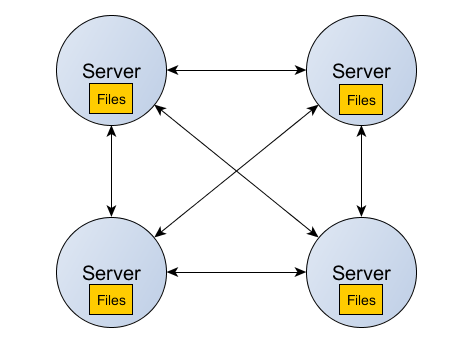
\includegraphics[scale=0.5]{images/architechure-diagram-server-server.png}
\caption{The highest level server-to-server system architecture}
\label{fig:highLvlNetwork}
\end{figure}

\clearpage


\section{Server to Client}

In the context of the local network of a single user, each of the client computers requiring data to be backed up
will connect to the server on that network. This server can be located anywhere within the network.
Upon the startup of each client, they each send a beacon to locate the server. The server and client
then make a connection and then secure it to allow the backup data to begin transferring. This relationship is reflected in Figure \ref{fig:indivNetwork}.

\begin{figure}[hb]
\centering
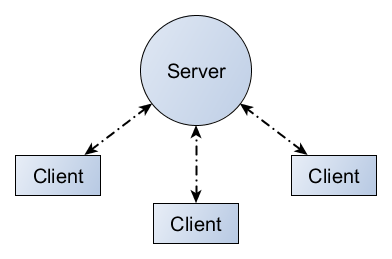
\includegraphics[scale=0.5]{images/architechure-diagram-server-client3.png}
\caption{The highest level server-to-server system architecture}
\label{fig:indivNetwork}
\end{figure}

\clearpage


\section{Server Architecture}

Figure \ref{fig:clientServer} details the internal structure of each individual server located on the user's LAN.  We see that each server has a connection into the larger P2P network of servers.  Also, each server connects to client machines on its LAN.  When a backup is initiated, either manually by a user or automatically according to scheduling, the Backup application on the server can start to retreive data from the client. Once the data and its form has been successfully stored, the Data Distributer is responsible for finding other backup servers and replicating the data to them.  When a user wishes to change the system's configuration, such as scheduling backup times or choosing which files to be backed up, they can access a Configuration web interface hosted on the server.  Finally, when the user wishes to restore, the Restore application is invoked, which takes data from the File Store and writes them back to the client.

\begin{figure}[hb]
\centering
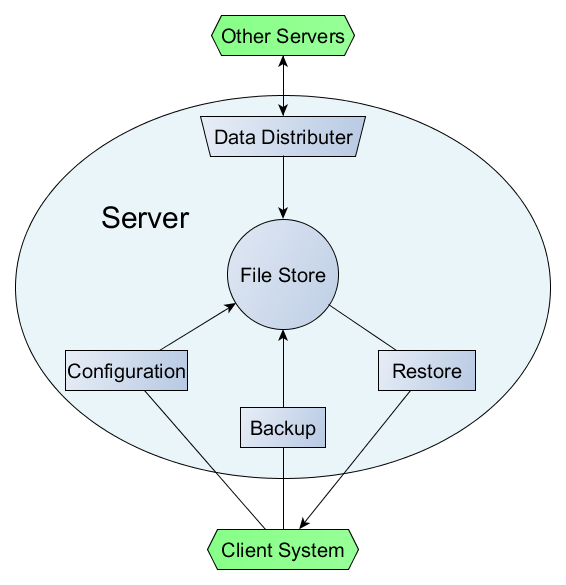
\includegraphics[scale=0.5]{images/architechure-diagram2.png}
\caption{A View of the Data Flow Through our Server}
\label{fig:clientServer}
\end{figure}